\documentclass[bachelor, och, labwork]{shiza}

\usepackage{subfigure}
\usepackage{tikz,pgfplots}
\pgfplotsset{compat=1.5}
\usepackage{float}
\usepackage{pdfpages}

\usepackage{titlesec}
\setcounter{secnumdepth}{4}
\titleformat{\paragraph}
{\normalfont\normalsize}{\theparagraph}{1em}{}
\titlespacing*{\paragraph}
{35.5pt}{3.25ex plus 1ex minus .2ex}{1.5ex plus .2ex}

\titleformat{\paragraph}[block]
{\hspace{1.25cm}\normalfont}
{\theparagraph}{1ex}{}
\titlespacing{\paragraph}
{0cm}{2ex plus 1ex minus .2ex}{.4ex plus.2ex}

% --------------------------------------------------------------------------%

\usepackage{multirow}
\usepackage[T2A]{fontenc}
\usepackage[utf8]{inputenc}
\usepackage{graphicx}
\graphicspath{ {./images/} }
\usepackage{tempora}

\usepackage[sort,compress]{cite}
\usepackage{amsmath}
\usepackage{amssymb}
\usepackage{amsthm}
\usepackage{fancyvrb}
\usepackage{listings}
\usepackage{listingsutf8}
\usepackage{longtable}
\usepackage{array}
\usepackage[english,russian]{babel}

\usepackage[hidelinks]{hyperref}
\usepackage{url}

\usepackage{underscore}
\usepackage{setspace}
\usepackage{indentfirst} 
\usepackage{mathtools}
\usepackage{amsfonts}
\usepackage{enumitem}
\usepackage{tikz}
\usepackage{minted}

\newcommand{\eqdef}{\stackrel {\rm def}{=}}
\newcommand{\specialcell}[2][c]{%
\begin{tabular}[#1]{@{}c@{}}#2\end{tabular}}

\renewcommand\theFancyVerbLine{\small\arabic{FancyVerbLine}}


\begin{document}
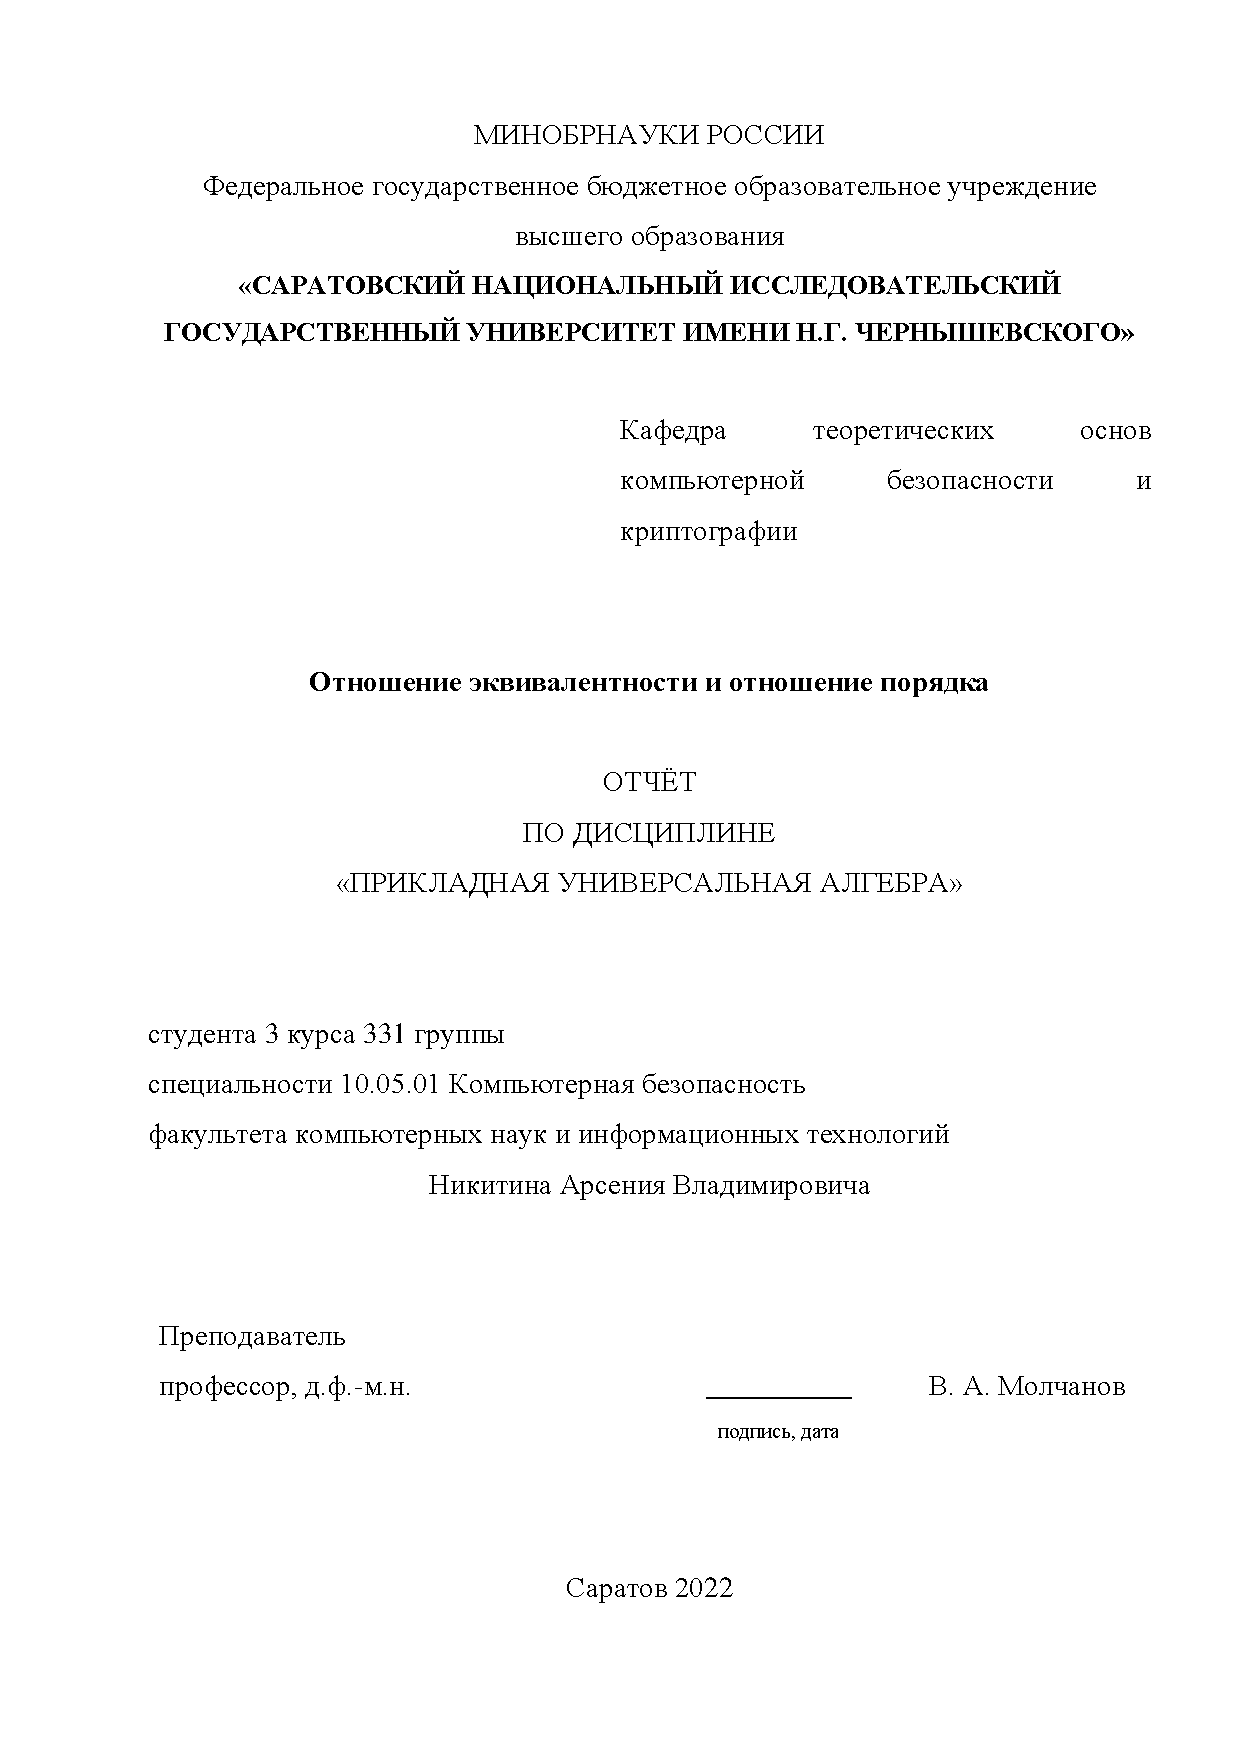
\includepdf{titul.pdf}

%-------------------------------------------------------------------------------

\tableofcontents

\intro

Бинарные отношения могут быть эквивалентными, и, поэтому на них могут строиться
фактор-множества. Если же бинарное отношение не является эквивалентностью, то
по определенному алгоритму можно построить эквивалентное замыкание данного
отношения. Также отношения могут обладать определенным порядком, в зависимости
от конкретных свойств. Если же отношение обладает порядком, то для данного
отношения можно построить диаграмму Хассе, а также для него могут быть
найдены минимальные и максимальные, и наименьшие и наибольшие элементы.
Также для бинарных отношений определены понятия контекста и концепта, а также
существует алгоритм вычисления решетки концептов.

\section{\textbf{Цель работы и порядок ее выполнения}}

\textbf{Цель работы} "--- изучение основных свойств бинарных отношений и 
операций замыкания бинарных отношений.

Порядок выполнения работы:

\begin{enumerate}

    \item Разобрать определения отношения эквивалентности, фактор-множества. 
    Разработать алгоритмы построения эквивалентного замыкания бинарного отношения 
    и системы представителей фактор-множества.  

    \item Разобрать определения отношения порядка и диаграммы Хассе. Разработать 
    алгоритмы вычисления минимальных (максимальных) и наименьших (наибольших) 
    элементов  и построения диаграммы Хассе. 

    \item Разобрать определения контекста и концепта. Разработать алгоритм 
    вычисления решетки концептов.

\end{enumerate}

\section{Теоретические сведения}

\subsection{Эквивалентное замыкание бинарного отношения}

\subsubsection{Системы замыканий бинарных отношений}

Множество $Z$ подмножеств множества $A$ называется \textbf{системой замыканий}, 
если оно замкнуто относительно пересечений, т.е. выполняется: \[\cap B \in Z ~\text{для любого подмножества}~ B \subset Z \]


\textit{Лемма о системах замыканий бинарных отношений.} На множестве $P(A^2)$ всех 
бинарных отношений между элементами множества $A$ следующие множества являются системами замыканий:

\begin{enumerate}
    \item $Z_r$ -- множество всех рефлексивных бинарных отношений между элементами множества $A$,
    \item $Z_s$ -- множество всех симметричных бинарных отношений между элементами множества $A$,
    \item $Z_t$ -- множество всех транзитивных бинарных отношений между элементами множества $A$,
    \item $Z_{eq} = Eq(A)$ -- множество всех отношений эквивалентности на множестве $A$.
\end{enumerate}

Множество $Z_{as}$ всех антисимметричных бинарных отношений между элементами множества $A$ не является системой замыкания.

\subsubsection{Замыкания бинарных отношений}
Итак, существуют 4 вида замыканий отношений: \textbf{транзитивное, симметричное, 
рефлексивное и эквивалентное}.

На множестве $P(A^2)$ всех бинарных отношений между элементами множества $A$ 
следующие отображения являются операторами замыканий:
\begin{enumerate}
    \item $f_r(\rho) = \rho ~\cup \vartriangle_A$ -- наименьшее рефлексивное
    бинарное отношение, содержащее отношение $\rho \subset A^2$. 
    \item $f_s(\rho) = \rho \cup \rho^{-1}$ -- наименьшее симметричное
    бинарное отношение, содержащее отношение $\rho \subset A^2$.
    \item $f_t(\rho) = \cup^{\infty}_{n=1} \rho^n$ -- наименьшее транзитивное
    бинарное отношение, содержащее отношение $\rho \subset A^2$.
    \item $f_{eq}(\rho) = f_tf_sf_r(\rho)$ -- наименьшее отношение эквивалентности,
    содержащее отношение $\rho \subset A^2$.
\end{enumerate}

\subsubsection{Алгоритм построения эквивалентного замыкания бинарного отношения}

\textit{Вход.} Матрица $M(\rho)$ бинарного отношения $\rho$ размерности
$N \times N$.

\textit{Выход.} Эквивалентное замыкание бинарного отношения.

\begin{enumerate}
    \item Создать пустой список для хранения пар замыкания.
    \begin{enumerate}[label=a)]
        \item Цикл по $u ~\text{от}~ 1 ~\text{до}~ N$.
        \begin{enumerate}[label=1.]\item Если $M_{uu} = 0$, пару $(u, u)$ добавить в замыкание.\end{enumerate} 
        \item Цикл по $k ~\text{от}~ 1 ~\text{до}~ N$.
        \begin{enumerate}[label=1.]\item Если $M_{uk} = 1 ~\text{и}~ M_{ku} = 0 $, пару $(k, u)$ добавить в замыкание.\end{enumerate}
        \item Цикл по $i ~\text{от}~ 1 ~\text{до}~ N$, цикл по $j ~\text{от}~ 1 ~\text{до}~ N$.
        \begin{enumerate}[label=1.]\item Если $M_{ki} = M_{ij} = 1 ~\text{и}~ M_{kj} = 0$, пару $(k, j)$ добавить в замыкание.\end{enumerate} 
    \end{enumerate}
    \item Ответ --- эквивалентное замыкание бинарного отношения $\rho$.
\end{enumerate}
Трудоемкость алгоритма $O(N^4)$

\subsection{Фактор-множество отношения}

\subsubsection{Определение среза отношения через элемент}
Для любого подмножества $X \subset A$ множество:
\begin{center} $\rho(X)=\{b \in B:(x,b)\in \rho ~\text{для некоторого}~ X\}$ \end{center}
называется \textit{образом} множества $X$ относительно отношения $\rho$.

Образ одноэлементного множества $X=\{a\}$ относительно отношения $\rho$
обозначается символом $\rho(a)$ и называется также образом элемента $a$ или
\textit{срезом} отношения $\rho$ через элемент $a$.

\subsubsection{Определение фактор-множества отношения}

Эквивалентное бинарное отношение на множестве $A$ также принято обозначать как
$\varepsilon$.

Срезы $\varepsilon(a)$ называются \textit{классами эквивалентности} по отношению
$\varepsilon$ и сокращенно обозначаются символом [$a$].

Множество всех таких классов эквивалентности $\{[a]:a\in A\}$ называется 
\textit{фактор-множеством} множества $A$ по эквивалентности $\varepsilon$ и 
обозначается $A/\varepsilon$.

\subsubsection{Алгоритм построения фактор-множества бинарного отношения}

\textit{Вход.} Матрица $M(\rho)$ эквивалентного бинарного отношения $\rho$ размерности
$N \times N$.

\textit{Выход.} Фактор-множество отношения.

\begin{enumerate}
    \item Создать пустое множество $S$.
    \begin{enumerate}[label=a)]
        \item Цикл по $i ~\text{от}~ 1 ~\text{до}~ N$
            \begin{enumerate} 
                \item Создать пустое множество $S_1$.
                \item Цикл по $j ~\text{от}~ 1 ~\text{до}~ N$.
                    \begin{enumerate}\item Если $M_{ij} = 1$, добавить $j$ во множество $S_1$.\end{enumerate}
                \item Добавить получившееся множество $S_1$ в $S$.
            \end{enumerate}
    \end{enumerate}
    \item Ответ --- фактор-множество отношения.
\end{enumerate}
    Трудоемкость алгоритма $O(N^2)$

\subsection{Полная система представителей классов эквивалентности}
\subsubsection{Определение полной системы представителей классов эквивалентности}
Подмножество $T\subset A$ называется \textit{полной системой представителей классов}
эквивалентности $\varepsilon$ на множестве $A$, если:
\begin{center}
    \begin{enumerate}
        \item $\varepsilon(T)=A$.
        \item из условия $t_1\equiv t_2(\varepsilon)$ следует $t_1=t_2$.
    \end{enumerate}
\end{center}
Классы эквивалентности $[t]\in A/\varepsilon$ могут быть отождествлены со своими
представителями $t$ и фактор-множество $A/\varepsilon$ может быть
отождествлено с множеством $T$.

\subsubsection{Алгоритм получения полной системы представителей классов эквивалентности}
\textit{Вход.} Матрица $M(\rho)$ эквивалентного бинарного отношения $\rho$ размерности
$N \times N$.

\textit{Выход.} Полная система представителей классов эквивалентности.
\begin{enumerate}
    \item Создать пустой список.
    \item Запустить алгоритм получения фактор-множества отношения.
    \item Цикл по $i$ от $1$ до количества элементов фактор-множества.
        \begin{enumerate} \item Добавить минимальный элемент $i$-го множества из фактор-множества в список.\end{enumerate}
    \item Ответ --- полная система представителей классов эквивалентности.
\end{enumerate}
Трудоемкость алгоритма -- $O(|S|)$

\subsection{Отношение порядка и упорядоченное множество}

Бинарное отношение $\omega$ на множестве $A$ называется \textit{отношением порядка}
(или просто \textit{порядком}), если оно рефлексивно, антисимметрично и транзитивно.

Поскольку отношение порядка интуитивно отражает свойство <<больше-меньше>>, то для
обозначения порядка $\omega$ используется инфиксная запись с помощью символа 
$\leq$: вместо $(a,b)\in \omega$ принято писать $a\leq b$.

Запись $a < b$ означает, что $a \le b$ и $a \not = b$.

Запись $a <\cdot b$ означает, что $a \le b$ и нет элементов $x$, удовлетворяющих
условию $a < x < b$. В этом случае говорят, что элемент $b$ \textit{покрывает} 
элемент $a$.

Элементы $a,b\in A$ называются \textit{сравнимыми}, если $a \le b$ или $b \le a$
или несравнимыми в противном случае.

\subsubsection{Определение упорядоченного множества}
Множество $A$ с заданным на нем отношением порядка $\le$ называется
\textit{упорядоченным множеством} и обозначается $A=(A,\le)$ или просто $(A,\le)$

\subsubsection{Определение минимальных (наименьших) и максимальных (наибольших) элементов упорядоченного множества}

Элемент $a$ упорядоченного множества $(A,\le)$ называется:
\begin{enumerate}
    \item \textit{минимальным}, если $(\forall x \in A) ~x \le a \Rightarrow x = a$
    \item \textit{максимальным}, если $(\forall x \in A) ~a \le x \Rightarrow x = a$
    \item \textit{наименьшим}, если $(\forall x \in A) ~a \le x$
    \item \textit{наибольшим}, если $(\forall x \in A) ~x \le a$
\end{enumerate}


\subsubsection{Определение диаграммы Хассе}

Упорядоченное множество $A = (A, \leq)$ наглядно представляется диаграммой Хассе, 
которая представляет элементы множества $A$ точками плоскости и пары $a <\cdot \text{ } b$ 
представляет линиями, идущими вверх от элемента $a$ к элементу $b$.

\subsubsection{Алгоритм построения диаграммы Хассе конечного упорядоченного множества}

\begin{center}\textit{Теоретический алгоритм}\end{center}
\begin{enumerate}
    \item В упорядоченном множестве $A = (A, \leq)$ найти множество $A_1$ всех минимальных элементов и расположить их в один горизонтальный ряд (это первый уровень диаграммы).
    \item В упорядоченном множестве $A \setminus A_1$, найти множество $A_2$ всех минимальных элементов и
    расположить их в один горизонтальный ряд над первым уровнем (это второй уровень диаграммы). Соединить
    отрезками элементы этого ряда с покрываемыми ими элементами предыдущего ряда.
    \item В упорядоченном множестве $A \setminus (A_1 \cup A_2)$ найти множество $A_3$ всех минимальных
    элементов и расположить их в один горизонтальный ряд над вторым уровнем (это третий уровень диаграммы).
    Соединить отрезками элементы этого ряда с покрываемыми ими элементами предыдущих рядов.
    \item Процесс продолжается до тех пор, пока не выберутся все элементы множества $A$.
\end{enumerate}

\begin{center}\textit{Псевдо-код алгоритма для множества с операцией деления}\end{center}

\textit{Вход}: Упорядоченное множество $A$ длиной $N$.

\textit{Выход}: Список $H$ длиной $n$, характеризующий диаграмму Хассе: каждый 
элемент в списке представляет собой три значения: элемент $a \in A$, значение его 
уровня $l$ на диаграмме, список $D$ элементов множества $A$, находящихся на 
уровне $l - 1$ и связанных с элементом $a$.

\begin{enumerate}
    \item Создать пустой список $H$.
    \item Создать словарь с ключами из элементов множества $A$ и значениями, равными 1.
    \item Цикл по $i$ от 2 до $N$.
        \begin{enumerate}
            \item Цикл по $j$ от 1 до $i$.
                \begin{enumerate}
                    \item Если $A_i$ делится на $A_j$, то элементу словаря
                    с ключом $A_i$ присвоить значение элемента словаря с ключом
                    $A_j$ + 1.
                \end{enumerate}
        \end{enumerate}
    \item Цикл по $key$, $value$ из словаря.
        \begin{enumerate}
        \item Создать пустой список $Q$.
        \item  Цикл по $key1$, $value1$ из словаря.
            \begin{enumerate}
                \item Если $value1 + 1 = value$ и $key$ делится на $key1$, то
                добавить $key1$ в $Q$. 
            \end{enumerate}    
        \item Добавить кортеж ($key,value,Q$) в список $H$.
        \end{enumerate}
    \item Ответ --- список, состоящий из элементов диаграммы Хассе, с уровнями 
    и связями с предыдущими уровнями диаграммы.
\end{enumerate}
Трудоемкость алгоритма --- $O(|A| * |A|) = O(|A|^2)$

\begin{center}\textit{Алгоритм получения делителей числа}\end{center}

\textit{Вход}: Число $a$.

\textit{Выход}: Список делителей числа $a$.
\begin{enumerate}
    \item Создать пустой список.
    \item Цикл по $i$ от 1 до $a/2+1$
        \begin{enumerate}
            \item Если $a$ делится на $i$, то добавить $i$ в список.
        \end{enumerate}
    \item Ответ --- список делителей числа $a$.
\end{enumerate}
Трудоемкость алгоритма --- $O(a/2+1)$

\begin{center}\textit{Псевдо-код алгоритма для множества, задаваемого числом с операцией деления}\end{center}

\textit{Вход}: Число $z$.

\textit{Выход}: Список $H$ длиной $n$, характеризующий диаграмму Хассе: каждый 
элемент в списке представляет собой три значения: элемент $a \in A$, значение его 
уровня $l$ на диаграмме, список $D$ элементов множества $A$, находящихся на 
уровне $l - 1$ и связанных с элементом $a$.

\begin{enumerate}
    \item Вызвать алгоритм получения делителей числа от $z$ и сохранить результат в список.
    \item Вызвать алгоритм получения элементов диаграммы Хассе для множества с операцией деления.
    \item Ответ --- список, состоящий из элементов диаграммы Хассе, с уровнями 
    и связями с предыдущими уровнями диаграммы.
\end{enumerate}
Трудоемкость алгоритма --- $O(|A| * |A|) = O(|A|^2)$, где $A$ -- множество всех
делителей числа $z$.

\subsubsection{Алгоритм получения минимальных элементов упорядоченного множества}

\textit{Вход}: Упорядоченное множество $A$ размерности $N$.

\textit{Выход.} Минимальные элементы множества $A$.
\begin{enumerate}
    \item Создать пустой список $R$ и добавить в него первый элемент кортежа
    первого элемента множества.
    \item Создать переменную $m_l$ и присвоить ей значение второго элемента кортежа
    первого элемента множества.
    \item Цикл по $i$ от 2 до $N$.
        \begin{enumerate}
            \item Если второй элемент кортежа $A_i$ равен $m_l$, то добавить
            первый элемент кортежа $A_i$ в $R$.
            \item Если второй элемент кортежа $A_i$ не равен $m_l$, то выход из цикла.
        \end{enumerate}
    \item Ответ --- минимальные элементы множества $A$: $R$
\end{enumerate}
Трудоемкость алгоритма --- $O(N)$.

\subsubsection{Алгоритм получения наименьшего элемента упорядоченного множества}
\textit{Вход}: Упорядоченное множество $A$ размерности $N$.

\textit{Выход.} <<Наименьшим элементом множества $A$ является $r$>> 
или <<Наименьшего элемента в данном множестве нет>>.
\begin{enumerate}
    \item Создать переменную $r$
    \item Вызвать алгоритм получения элементов диаграммы Хассе для множества с операцией деления.
    \item Если вторые элементы кортежей (отвечающие за уровень элемента) первого
    и второго элемента полученного множества равны, то ответ --- <<Наименьшего элемента в данном множестве нет>>.
    \item Если вторые элементы кортежей первого и второго элемента полученного 
    множества различны, то $r$ присвоить значение первого элемента первого кортежа.
    Ответ --- <<Наименьшим элементом множества $A$ является $r$>>.
\end{enumerate}
Трудоемкость алгоритма --- $O(1)$

\subsubsection{Алгоритм получения максимальных элементов упорядоченного множества}
\textit{Вход}: Упорядоченное множество $A$ размерности $N$.

\textit{Выход.} Максимальные элементы множества $A$.
\begin{enumerate}
    \item Создать пустой список $R$ и добавить в него первый элемент кортежа
    последнего элемента множества.
    \item Создать переменную $m_l$ и присвоить ей значение второго элемента кортежа
    последнего элемента множества.
    \item Цикл по $i$ от $N-1$ до $1$.
        \begin{enumerate}
            \item Если второй элемент кортежа $A_i$ равен $m_l$, то добавить
            первый элемент кортежа $A_i$ в $R$.
            \item Если второй элемент кортежа $A_i$ не равен $m_l$, то выход из цикла.
        \end{enumerate}
    \item Ответ --- максимальные элементы множества $A$: $R$
\end{enumerate}
Трудоемкость алгоритма --- $O(N)$.

\subsubsection{Алгоритм получения наибольшего элемента упорядоченного множества}
\textit{Вход}: Упорядоченное множество $A$ размерности $N$.

\textit{Выход.} <<Наибольшим элементом множества $A$ является $r$>> 
или <<Наибольшего элемента в данном множестве нет>>.
\begin{enumerate}
    \item Создать переменную $r$
    \item Вызвать алгоритм получения элементов диаграммы Хассе для множества с операцией деления.
    \item Если вторые элементы кортежей (отвечающие за уровень элемента) последнего
    и предпоследнего элемента полученного множества равны, то ответ --- <<Наибольшего элемента в данном множестве нет>>.
    \item Если вторые элементы кортежей первого и второго элемента полученного 
    множества различны, то $r$ присвоить значение первого элемента первого кортежа.
    Ответ --- <<Набольшим элементом множества $A$ является $r$>>.
\end{enumerate} 
Трудоемкость алгоритма --- $O(1)$

\subsection{Контексты и решетки концептов}
Бинарное отношение $\rho \subset G\times M$ между элементами множеств $G$ и $M$
можно рассматривать как базу данных с множеством объектов $G$ и множеством
атрибутов $M$. Такая система называется также контекстом и определяется следующим
образом.

\textit{Контекстом} называется алгебраическая система $K=(G,M,\rho)$, состоящая
из множества \textit{объектов} $G$, множества \textit{атрибутов} $M$ и бинарного
отношения $\rho \subset G\times M$, показывающего $(g,m)\in\rho$, что объект $g$
имеет атрибут $m$.

Контекст $K = (G,M,\rho)$ наглядно изображается таблицей, в которой строки
помечены элементами множества $G$, столбцы помечены элементами множества $M$ и
на пересечении строки с меткой $g \in G$ и столбца с меткой $m \in M$ стоит 
элемент:
\begin{equation*}
    k_{g,m} = 
        \begin{cases}
            1, &\text{если $(g,m) \in \rho$}\\
            0, &\text{если  $(g,m) \not\in \rho$}
        \end{cases}
\end{equation*}

Упорядоченная пара $(X,Y)$ замкнутых множеств $X\in Z_{f_G}$, $Y\in Z_{f_M}$,
удовлетворяющих условиям $\varphi(X)=Y, \psi(Y)=X$, называется \textit{концептом}
контекста $K=(G,M,\rho)$. При этом компонента $X$ называется \textit{объемом} и
компонента $Y$ --- содержанием концепта $(X,Y)$.

Множество всех концептов $C(K)$ так упорядочивается отношением $(X,Y)\le(X_1,Y_1) \Leftrightarrow X \subset X_1$
(или равносильно $Y_1 \subset Y$), что $(C(K),\le)$ является полной решеткой,
которая изоморфна решетке замкнутых подмножеств $G$.

\subsubsection{Алгоритм вычисления системы замыканий на множестве $G$}
\begin{enumerate}
    \item Рассматриваем множество $G \in Z_{f_G}$.
    \item Последовательно перебираем все элементы $m \in M$ и вычисляем для них $\psi(\{m\}) = \rho^{-1}(m)$.
    \item Вычисляем все новые пересечения множества $\psi(\{m\})$ с ранее полученными множествами и добавляем новые множества к $Z_{f_G}$. Аналогично вычисляется система замыканий на множестве $M$.
\end{enumerate}

\subsubsection{Алгоритм получения элементов решетки концептов}
\textit{Вход}: Матрица бинарного отношения $M(\rho)$ размерности $N\times N$,
множество атрибутов $A$.

\textit{Выход.} Решетка концептов.

\begin{enumerate}
    \item Создать пустое множество $c_s$, множество $a_s$, заполненного числами
    от 1 до $N$, пустой словарь $s_a$.
    \item Цикл по $i$ от 1 до $N$.
        \begin{enumerate}
            \item Создать пустое множество $n_s$.
            \item Цикл по $j$ от 1 до $N$.
                \begin{enumerate}\item Если $M(\rho)_{ij}=1$, добавить $j$ в $n_s$.\end{enumerate}
            \item Присвоить $a_s$ пересечение $a_s$ и $n_s$.
            \item Если множество $c_s$ пустое:
                \begin{enumerate}
                \item Добавить $n_s$ в $c_s$.
                \item В словаре $s_a$ по ключу $A[i]$ присвоить значение $n_s$. 
                \end{enumerate} 
            \item Создать пустое множество $s$.
            \item Цикл по элементам $u$ из множества $c_s$.
                \begin{enumerate}
                    \item Создать множество $ss$ и присвоить ему пересечение 
                    $u$ с $n_s$.
                    \item Если множество $ss$ непустое:
                        \begin{enumerate}
                            \item Цикл по $key,value$ в словаре $s_a$:
                                \begin{itemize}
                                    \item Если $value=u$, в словаре $s_a$ по ключу $key, A[i]$ присвоить значение $ss$, выход из цикла.
                                \end{itemize}
                            \item Во множество $s$ добавить множество $ss$.
                        \end{enumerate}
                \end{enumerate}
           \item Цикл по элементам $u$ из множества $s$.
                \begin{enumerate}\item Во множество $c_s$ добавить множество $u$.\end{enumerate}
            
            \item Если множество $n_s$ не находится во множестве $c_s$, во множество $c_s$ добавить множество $n_s$
                  и в словаре $s_a$ по ключу $A[i]$ присвоить значение $n_s$.
        \end{enumerate}
    \item Создать переменную $s_g =\varnothing$.
    \item Цикл по $key,value$ в словаре $s_a$:
        \begin{enumerate} \item Если $value=a_s$, $s_g = value$, выход из цикла.\end{enumerate}
    \item Ответ --- решетка концептов.
\end{enumerate}
Трудоемкость алгоритма --- $O(N^3 + N^2 + N^1) = O(N^3)$

\section{Программная реализация рассмотренных алгоритмов}
    
    \subsection{Результаты тестирования программы}

        \begin{figure}[H]
            \centering
            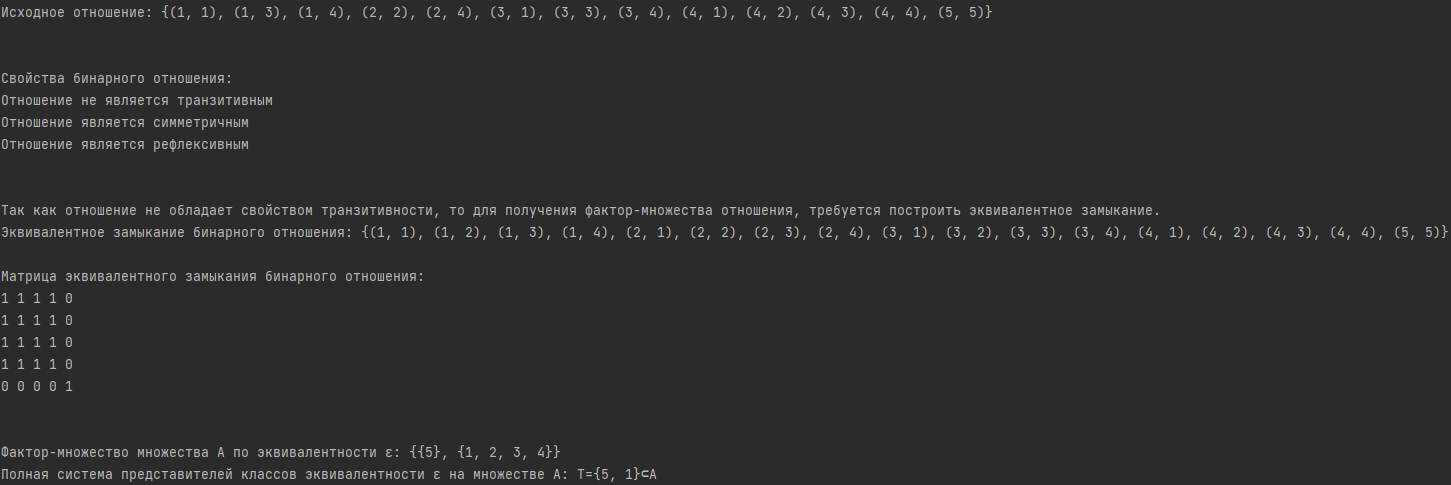
\includegraphics[width=0.8\textwidth]{pic/1.png}
            \caption{}
        \end{figure}

        
        \begin{figure}[H]
            \centering
            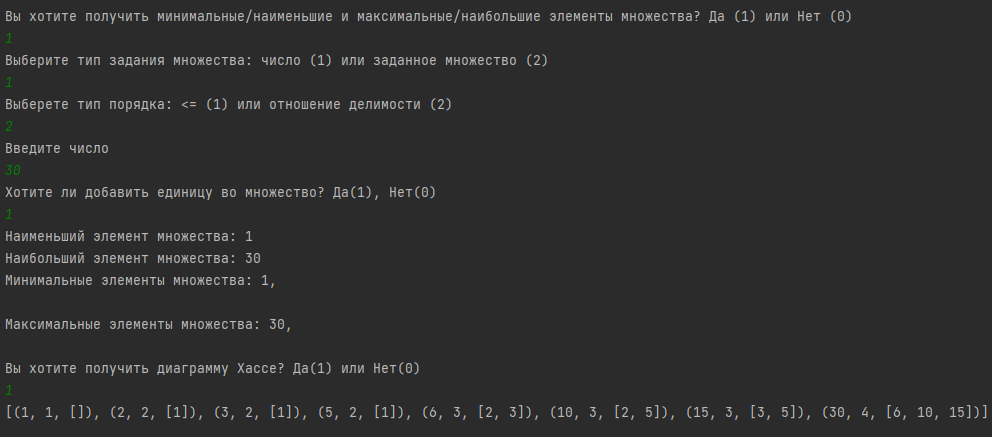
\includegraphics[width=0.8\textwidth]{pic/2.png}
            \caption{}
        \end{figure}

        
        \begin{figure}[H]
            \centering
            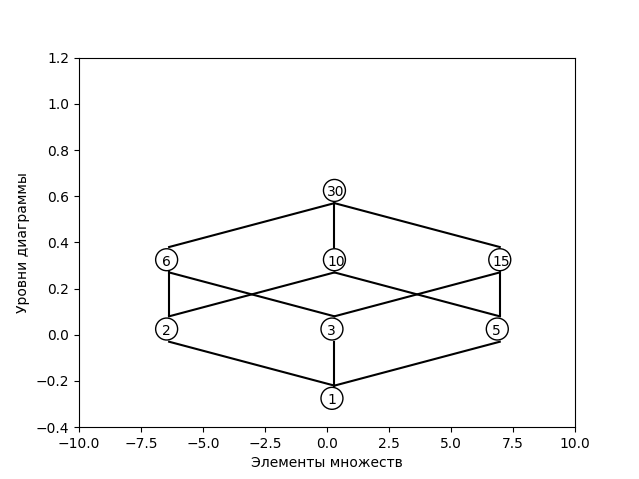
\includegraphics[width=0.8\textwidth]{pic/3.png}
            \caption{}
        \end{figure}

        \begin{figure}[H]
            \centering
            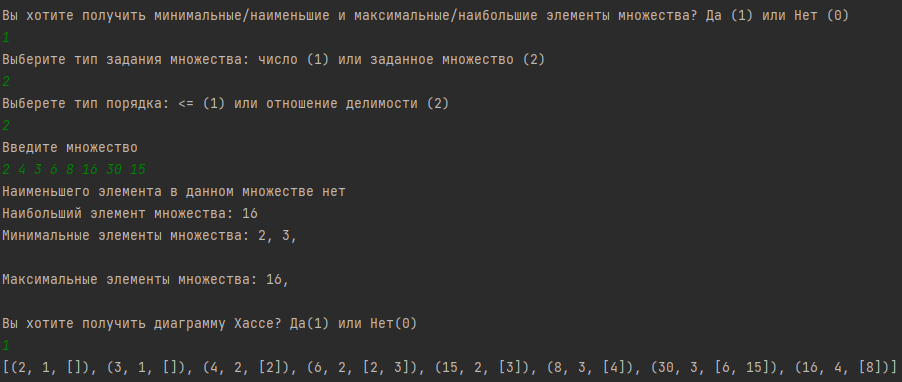
\includegraphics[width=0.8\textwidth]{pic/4.png}
            \caption{}
        \end{figure}

        \begin{figure}[H]
            \centering
            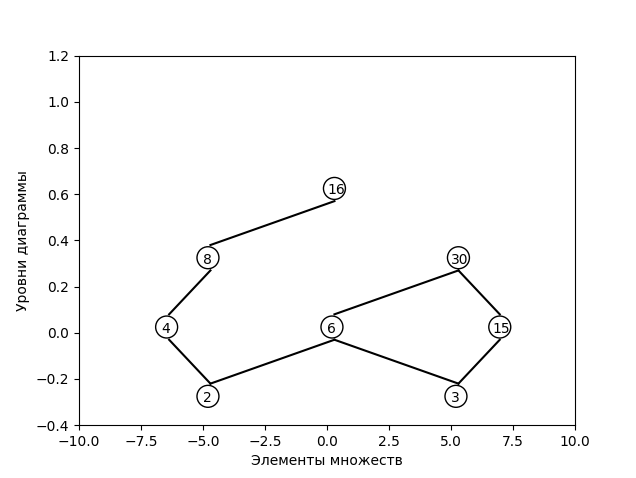
\includegraphics[width=0.8\textwidth]{pic/5.png}
            \caption{}
        \end{figure}

        \begin{figure}[H]
            \centering
            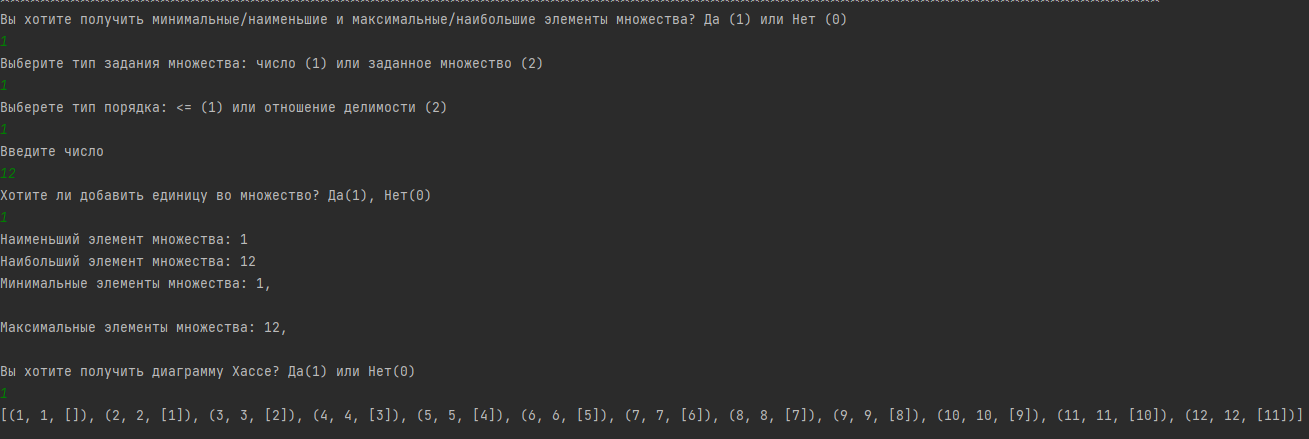
\includegraphics[width=0.8\textwidth]{pic/6.png}
            \caption{}
        \end{figure}

        \begin{figure}[H]
            \centering
            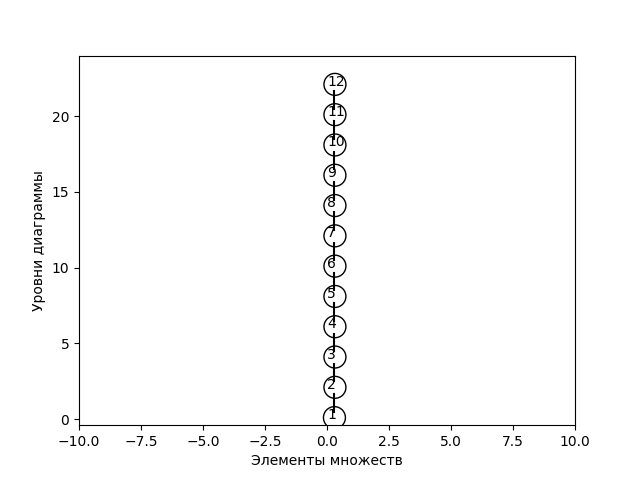
\includegraphics[width=0.8\textwidth]{pic/7.png}
            \caption{}
        \end{figure}

        \begin{figure}[H]
            \centering
            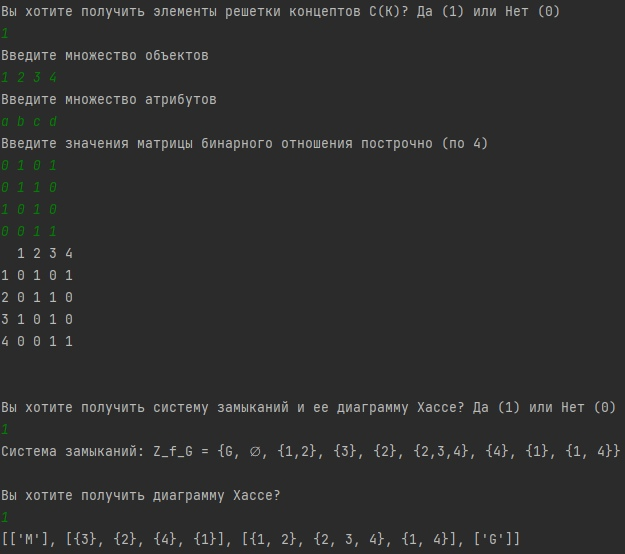
\includegraphics[width=0.8\textwidth]{pic/8.png}
            \caption{}
        \end{figure}
    
    \subsection{Коды программ, реализующих рассмотренные алгоритмы}
    \setminted[python]{linenos,breaklines=true, fontsize=\small, style=bw}
        \subsubsection{Код программы, реализующей визуализацию диаграммы Хассе}
            \inputminted{python}{code/hassevisualization.py}
        \subsubsection{Код программы, реализующей получение решетки концептов}
            \inputminted{python}{code/latticeofconcepts.py}
        \subsubsection{Код программы, реализующей основные алгоритмы}
            \inputminted{python}{code/lab2.py}
      


\conclusion
В ходе лабораторной работы были рассмотрены понятия эквивалентного замыкания
бинарного отношения и получения представителей фактор-множества. Также были
получены алгоритмы вычисления минимальных и максимальных, и наименьших и наибольших
элементов бинарного отношения, а также был определен и программно реализован
алгоритм построения диаграммы Хассе. Был описан алгоритм построения решетки
концептов. Для всех алгоритмов произведена асимптотическая оценка.
\end{document}